%!TEX root = FreeRtos ARM uController.tex
\subsection{Zielsysteme STM32F4 (ARM Cortex M4)}
Der STM32F4 ist ein von STMicroelectronics entwickelter 32 Bit uController basierend auf einem ARM Cortex M4 Kern. Der STM32F4 läuft auf maximal 168 Mhz. Neben seinen unzähligen Schnittstellen (4x UART, SPI, I2C, Ethernet) bietet der STM32F4 mehrere Energiespar-Modis, die ihn für den Einsatz in energieeffiziente Anwendung wie IOT Devices interessant machen. Für die Verwendung von FreeRTOS eignet sich der uController besonders gut, da speziell für diesen uController viele Hardware-Funk\-tio\-na\-li\-tät\-en in den FreeRTOS Kernel integriert wurden. Der STM32F4 ist seit 2012 auf dem Markt und erfährt durch eine große Anzahl an online Beispielen eine hohe Beliebtheit in der Entwickler Community. Zum Zugriff auf uController Funktionen stellt STM das Hardware Abstraction Layer kurz HAL zur Verfügung, sie Abbildung \ref{fig:HAL}. Die HAL ermöglicht eine einfache Verwendung der Hardware ohne großen Konfigurationsaufwand.     
\begin{figure}[htb!]
	\centering
		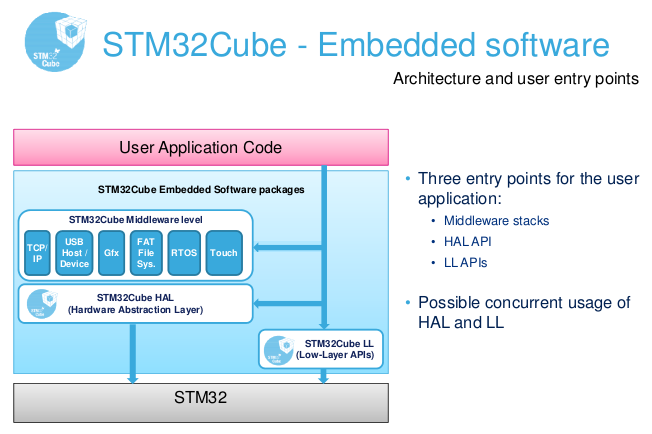
\includegraphics[width=0.4\textwidth]{Pictures/STM32F4/LibraryEntry.png}
	\caption{Aufbau der zur Verfügung stehenden STM Bibliotheken }
	\label{fig:HAL}
\end{figure}
Wie spezielle Hardware-Funktionen des STM32F4 durch FreeRTOS genutzt werden können, wird in Abschnitt \ref{sec:Low Power Modes} und Abschnitt \ref{sec:Memory Protection} gezeigt.